% !TEX root = ../document.tex

\chapter{现阶段发展及应用情况}

\section{DLR 的 AOS 实验项目}

\subsection{项目概述}

根据\ref{sec:space_based_ads-b_experiment_back}节的内容,我们得知 DLR 的 AOS(ADS-B over Satellite)项目是世界上第一个天基 ADS-B 可行性验证实验项目。AOS 开发了一个 ADS-B 载荷,作为一个在轨演示器,搭载在 ESA(欧洲航天局)的 PROBA-Vegetation 卫星上,于 2013 年 5 月 7 日被发射到近地轨道上。AOS 是 DLR 空间系统研究所和 DLR 飞行指导研究所的合作项目,与卢森堡合作伙伴 SES TechCom Services 合作。

\renewcommand\arraystretch{1.5}
\begin{table}[htbp]
\centering
\caption{DLR 的 AOS 项目基本描述}
\label{tab:}
\begin{tabular}[b]{|p{2.5cm}<{\raggedleft}|p{12cm}<{\raggedright}|}
\hline
\textbf{目标} & 证明星基 ADS-B 监视的可行性 \par
            搭载于 ESA 的 Proba-V 卫星上的在轨演示器将验证一些关键参数,例如目标截获率、检测率和验证概率 \\
\hline
\textbf{项目持续时间} & 2011 年第一季度至 2014 年第二季度末 \\
\hline
\textbf{合作方} & Institute of Space Systems (RY) in Bremen, Germany \par
        Institute for Flight Guidance (FL) in Braunschweig, Germany \\
\hline
\textbf{贡献} & Institute RY: 开发和组装符合空间要求的 ADS-B 接收机和天线\par
Flight Calibration Services: 开发 ADS-B 接收机\par
Institute FL: ADS-B 数据的验证与评估 \\
\hline
\textbf{更多的合作} & RY with SES-ASTRA / ESA: 提供数据服务器 \\
\hline
\end{tabular}
\end{table}

\renewcommand\arraystretch{1.5}
\begin{table}[htbp]
\centering
\caption{ESA 的 Proba-V 小卫星任务描述}
\label{tab:esa_Proba-V_mission}
\begin{tabular}[b]{|p{2.5cm}<{\raggedleft}|p{12cm}<{\raggedright}|}
\hline
\textbf{主承包商} & QinetiQ Space nv \\
\hline
\textbf{卫星质量} & 约 140kg\\
\hline
\textbf{运载火箭 }& Vega 火箭\\
\hline
\textbf{发射日期} & 2013 年 5 月 7 日 \\
\hline
\textbf{发射场} & 法属圭亚那航天中心(库鲁)\\
\hline
\textbf{发射提供商} & Arianespace \\
\hline
\textbf{轨道} & 太阳同步轨道,海拔 820 公里,倾角 98.73$^\circ$,飘移限制在 10:30AM 到 11:30AM  \\
\hline
\textbf{通信} & 卫星的控制与通信通过比利时 Redu 地面站 \\
\hline
\textbf{主要任务} & 植被扫描仪 \\
\hline
\textbf{载荷} & ADS-B、高能粒子传感器、氮化镓 X 波段功率放大器 \\
\hline
\end{tabular}
\end{table}

ESA Proba-V 卫星自 2013 年 5 月 7 日起进入地球轨道, 其有效载荷包括一个专用接收器,用于接收飞机 ADS-B 信号。5 月 23 日,该实验首次开启,在两小时内在 820 公里的高度记录了 12000 条 ADS-B 信息。飞越苏格兰的 A320 飞机是 DLR 新型接收机从太空“看到”的第一架飞机,证明可以从太空跟踪飞机。


\subsection{体系结构}

Proba-V 上的 ADS-B 接收器由卢森堡的 DLR 和 SES TechCom 提供,主要目的是在飞行代表性配置中测试(空间限定)ADS-B 电路板以评估 TID(总电离剂量)。

ADS-B 接收器(1090ES RX)的基本设计概念是单转换超外差接收机,由 1090MHz 下变频调至中频 70MHz,70MHz 下的 IF 采样由一个 105Msps(每秒兆采样次数)的 16 位 ADC 完成。该 ADS-B 单转换超外差接收机概念如图\ref{fig:dlr_ads-b_receiver}所示\upcite{e2}。

\begin{figure}[htbp]
\centering
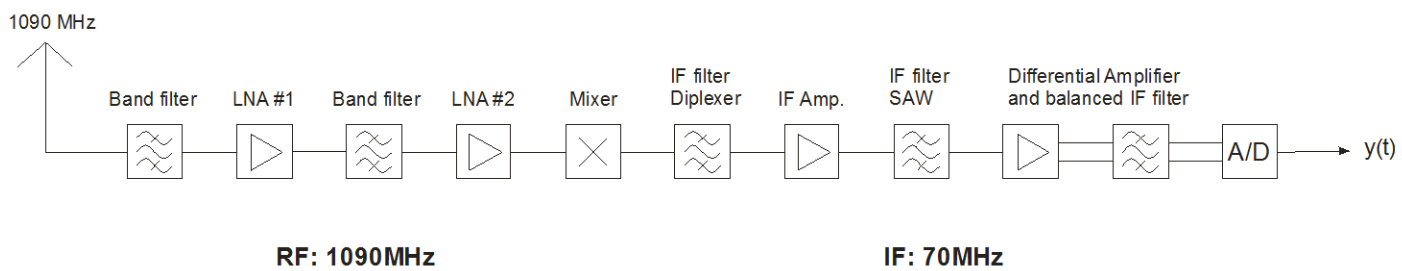
\includegraphics[width=15cm]{pic/dlr_ads-b_receiver.png}
\caption{单转换超外差接收机}
\label{fig:dlr_ads-b_receiver}
\end{figure}

\begin{figure}[htbp]
\centering
\subfigure[载荷原型]{
\begin{minipage}[b]{0.3\linewidth}
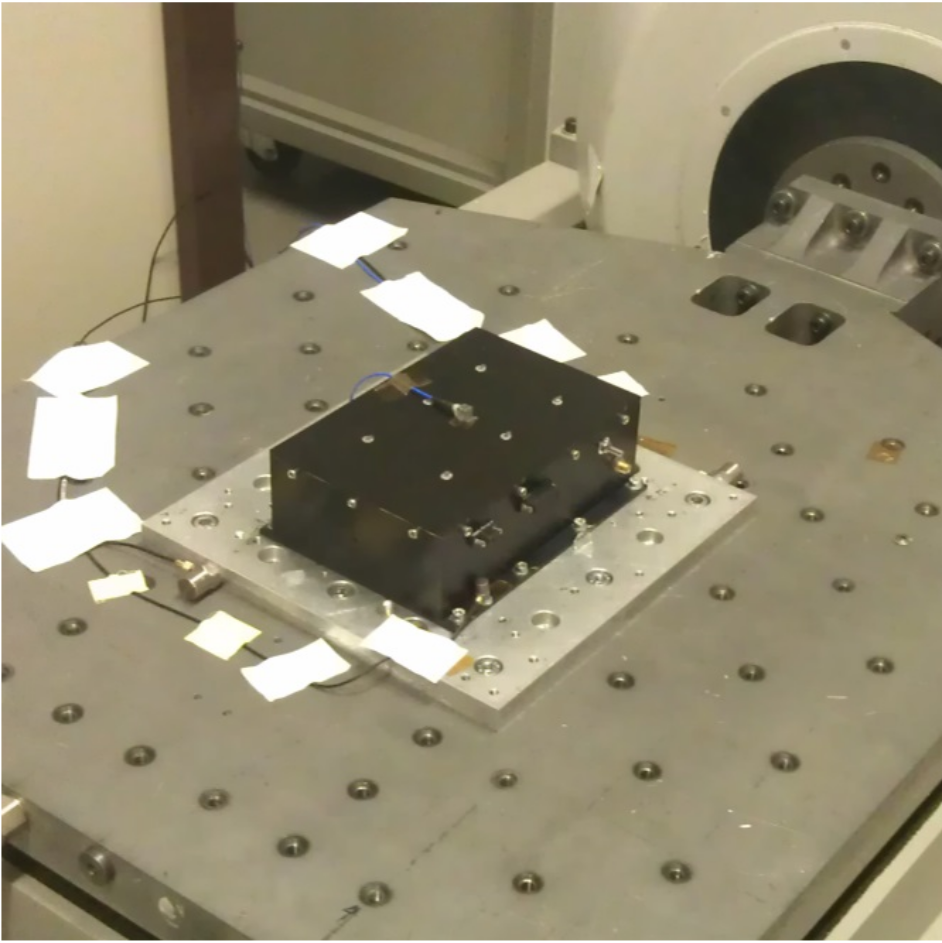
\includegraphics[width=1\linewidth]{pic/aos_ads-b_payload_2.png}
\end{minipage}}
\subfigure[安装位置]{
\begin{minipage}[b]{0.3\linewidth}
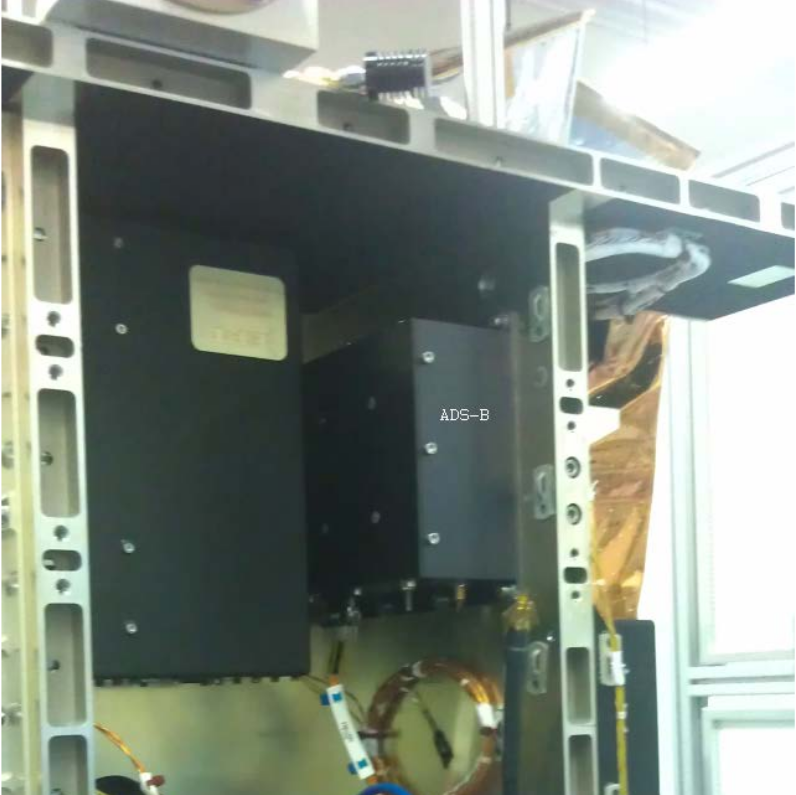
\includegraphics[width=1\linewidth]{pic/aos_ads-b_payload_1.png}
\end{minipage}}
\subfigure[卫星原型]{
\begin{minipage}[b]{0.3\linewidth}
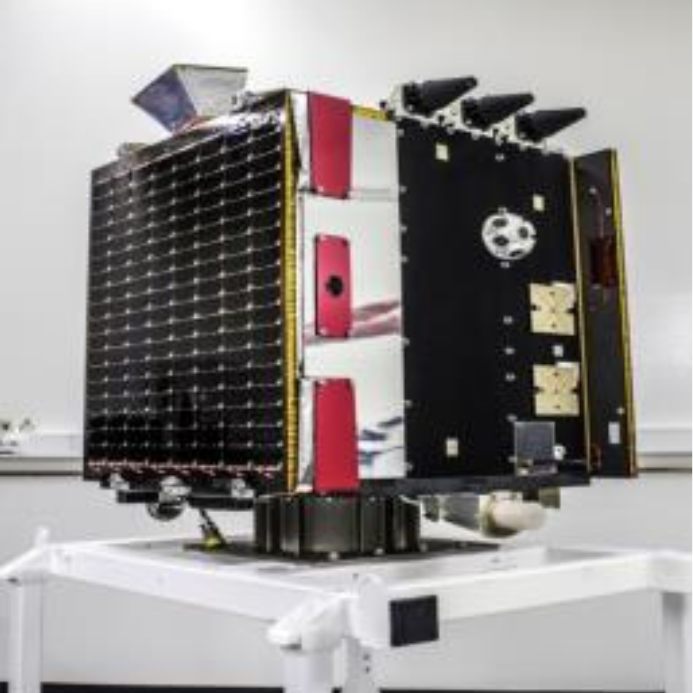
\includegraphics[width=1\linewidth]{pic/aos_ads-b_payload_3.png}
\end{minipage}}
\caption{Proba-V 卫星上搭载的 ADS-B 载荷}
\label{fig:aos_ads-b_payload}
\end{figure}

\begin{figure}[htbp]
\centering
\begin{minipage}[t]{0.48\textwidth}
\centering
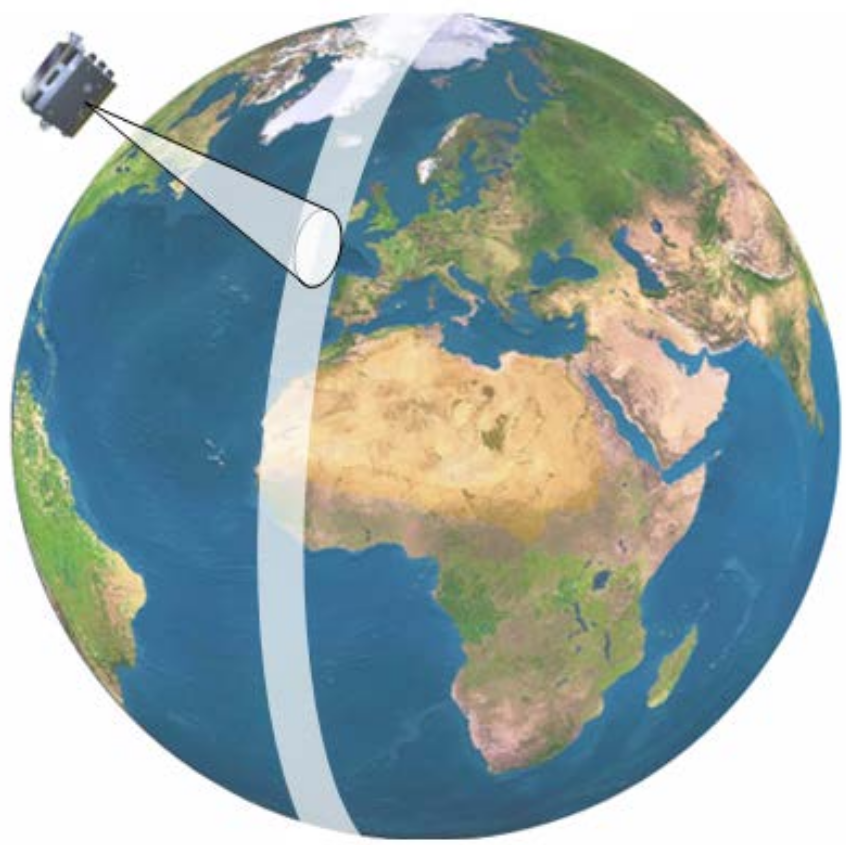
\includegraphics[width=6cm]{pic/aos_in_orbit.png}
\caption{技术验证阶段的单颗卫星}
\label{fig:aos_in_orbit}
\end{minipage}
\begin{minipage}[t]{0.48\textwidth}
\centering
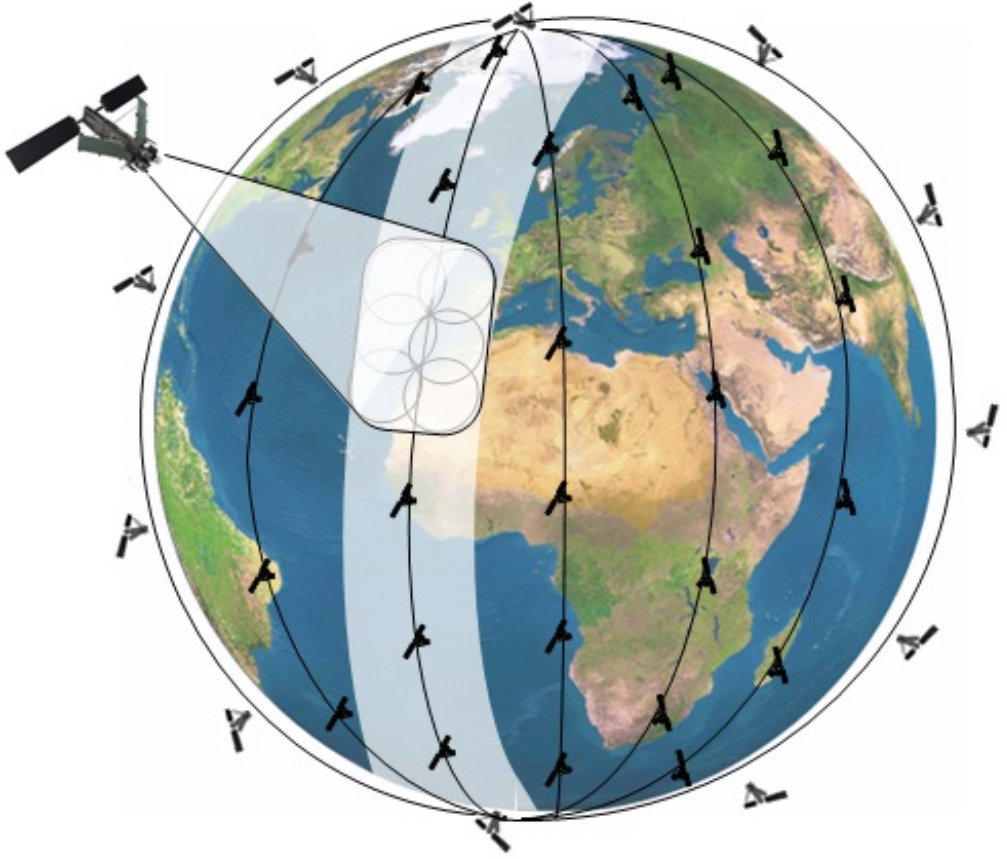
\includegraphics[width=7.2cm]{pic/aos_in_future.png}
\caption{未来全球卫星组网方案}
\label{fig:aos_in_future}
\end{minipage}
\end{figure}

\subsection{实验结果}

图\ref{fig:ADS-B_Auto6}展示了 2014 年 2 月 11 日在世界范围内记录的飞机航迹,每个红点代表卫星在其轨道上通过飞机时所看到的飞机航迹段。Proba-V 卫星的天线覆盖范围为纵向约 1200 公里,横向延伸至卫星飞行方向 500 公里,可逐条扫描全球空域。

\begin{figure}[htbp]
\centering
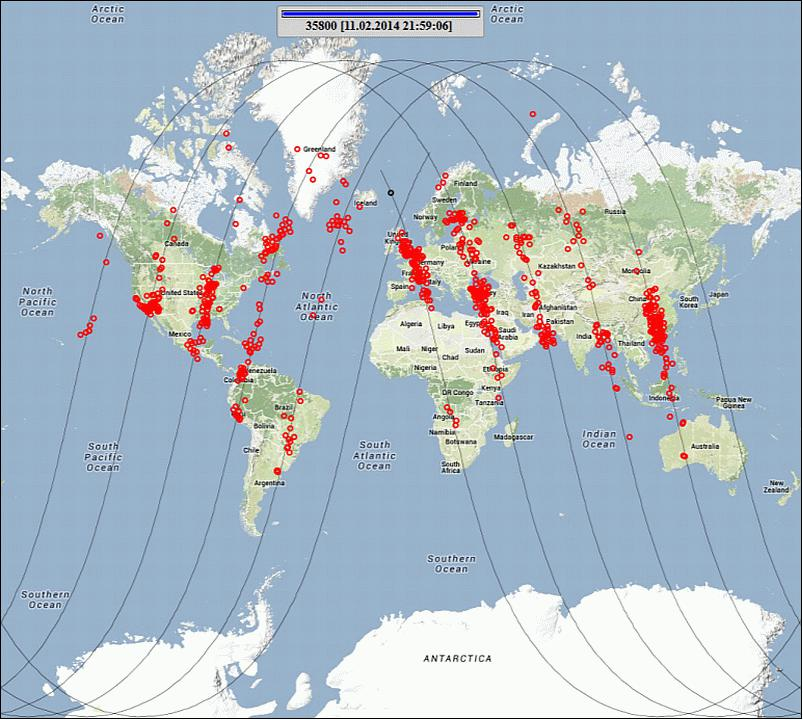
\includegraphics[width=10cm]{pic/ADS-B_Auto6.jpeg}
\caption{AOS 在世界范围内记录的飞机航迹(2014 年 2 月 11 日)}
\label{fig:ADS-B_Auto6}
\end{figure}

在空间接收 ADS-B 报文的最重要方面是卫星上 1090 MHz 扩展电文信号的接收条件。与基于地面的 ADS-B 监视相比,陆基 ADS-B 最大接收范围可达 300 公里,而在 820 公里高度轨道运行的 LEO 卫星与飞机之间的信号路径要长得多,这导致 ADS-B 的信号电平较低。接收器必须通过相关处理几乎在噪声水平上检测 S 模式信号。

实验得到了卫星天线覆盖区中不同区域接收到的 ADS-B 报文数量分布的直方图,如图\ref{fig:ADS-B_Auto5}所示,该图显示了 2014 年 5 月收到的所有位置消息的直方图。值得注意的是两个峰值,一个在卫星运动方向前方,峰值较低,另一个在卫星运动方向后方,峰值较高。这个谱的分布是不对称的,这由许多原因引起,比如卫星上的贴片天线的安装位置不对称、安装在卫星下侧的其他设备和在下表面的前边缘上突出的太阳能电池板。

\begin{figure}[htbp]
\centering
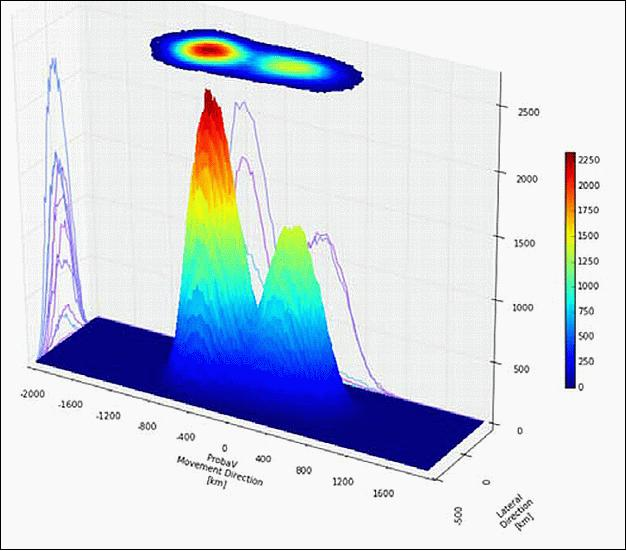
\includegraphics[width=10cm]{pic/ADS-B_Auto5.jpeg}
\caption{所有接收到的位置信息在天线覆盖区中的分布直方图}
\label{fig:ADS-B_Auto5}
\end{figure}

直方图的峰值可以通过卫星的接收天线和飞机的发射天线的天线辐射图来解释。图\ref{fig:ADS-B_Auto4}显示了安装在 Proba-V 卫星最低点面板上的 ADS-B 贴片天线的实测辐射图。合成的天线辐射图在卫星移动方向整体呈椭圆形状,最大灵敏度略低于卫星下方的最低点方向。

飞机装有两个 ATC 天线,一个在机身顶部,一个在机身底部,它们交替发射。由于几何因素限制,卫星将接收来自顶部天线的信号。顶部天线典型的垂直天线辐射模式如图\ref{fig:antenna_of_plane}所示。

\begin{figure}[htbp]
\centering
\begin{minipage}[t]{0.48\textwidth}
\centering
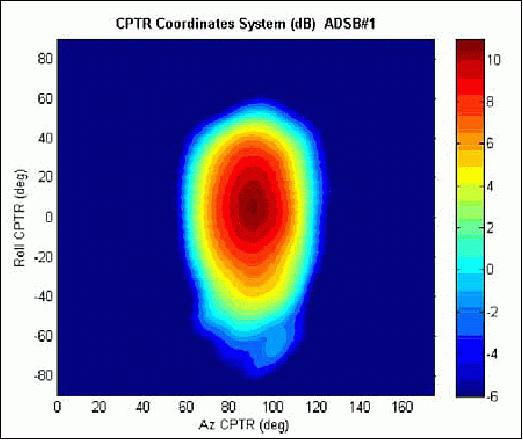
\includegraphics[width=7.5cm]{pic/ADS-B_Auto4.jpeg}
\caption{Proba-V 卫星天线辐射图}
\label{fig:ADS-B_Auto4}
\end{minipage}
\begin{minipage}[t]{0.48\textwidth}
\centering
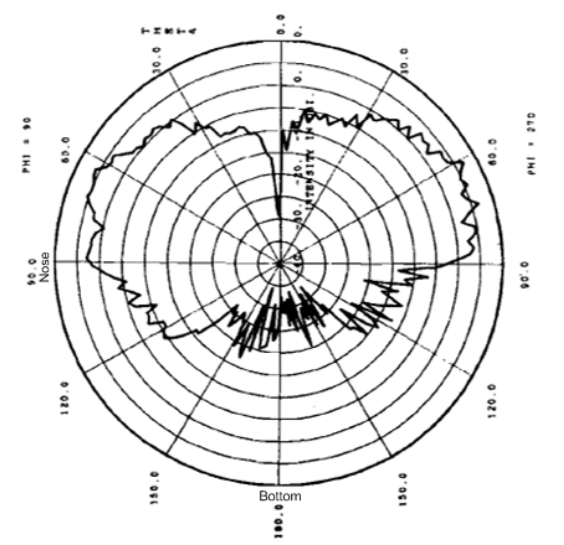
\includegraphics[width=6.5cm]{pic/antenna_of_plane.png}
\caption{顶部安装的 L 波段天线的垂直天线辐射图}
\label{fig:antenna_of_plane}
\end{minipage}
\end{figure}

\subsection{项目意义}

这次星载 ADS-B 接收验证实验的创举,将带来更多的在轨验证任务。ESA 与 Thales 德国签订合同,开发下一代 ADS-B 系统,该系统正在按计划进行,同时带来了卢森堡航天界(如 LuxSpace)的大力参与,将 TRITON 微小卫星平台作为以后的实验平台\upcite{h2}。

Proba-V 卫星实验项目取得了多个成果,主要包括:

\begin{itemize}
    \item 接收器的 FPGA 固件中包含一项特殊功能:允许上载新配置文件并通过远程访问激活这些配置。到目前为止,在任务运行期间,已成功测试了几次;

    \item 开发了改进的 S 模式相关机制,这得益于脉冲序列从第一个到第五个前导脉冲的相位相干性。在实验室测试中,可以显示报文检测率显著增加;

    \item 通过为 DF17 中的 112 个 S 模式数据位生成并保存“低置信度位”,增加了一次可以提高后处理报文解调成功率的机会;

    \item 卫星上的 ADS-B 接收器是同类中的第一个实验,接收从飞机发射的 1090ES ADS-B 电文信号。因此无法根据以往经验或任何结果进行系统设计。
\end{itemize}

Proba-V 卫星在实验中也遇到了一些困难,主要包括:

\begin{itemize}
    \item 由于卫星在大约 820 公里的高度,而飞机在 0 到 12 公里的高度,距离会导致接收的信号幅度过低从而导致信号丢失;

    \item 由于卫星天线垂直辐射图和飞机天线垂直辐射图的形状不同,会导致信号损失;

    \item 当到达卫星 ADS-B 天线的消息在时间上重叠(交织)时,ADS-B 接收机无法对其进行解码;

    \item 卫星的速度约为 27000 公里/小时,这导致每个检测到的飞机的观察时间有限,最多约 3 分钟。
\end{itemize}

这些困难提供了巨大的借鉴意义,为星基 ADS-B 技术发展中探明了一些需要克服的难点问题。

\section{Aireon 星基 ADS-B 系统}

\subsection{系统概述}



\begin{figure}[htbp]
\centering
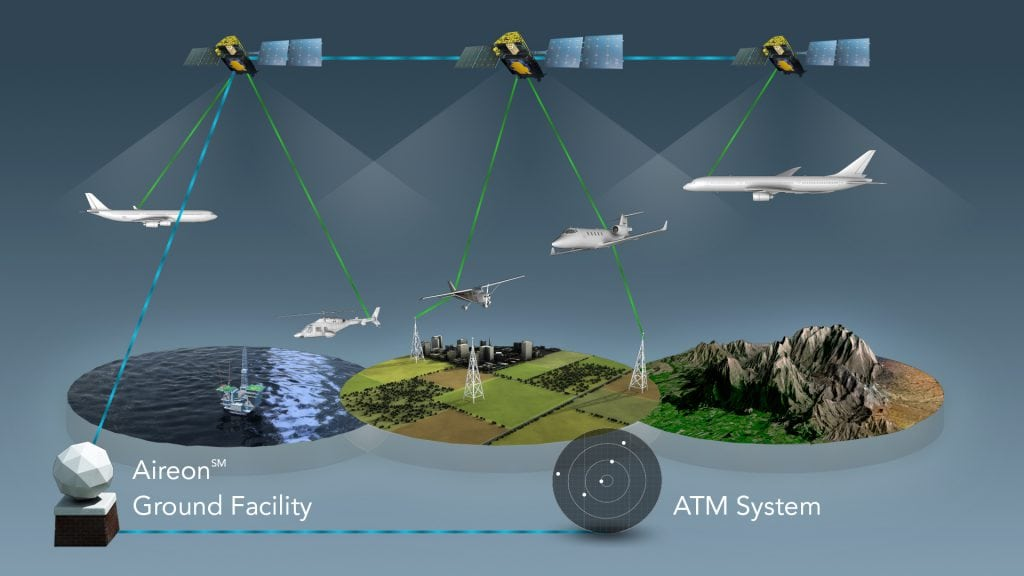
\includegraphics[width=15cm]{pic/Aireon_GlobalSpaceBasedADSB_Coverage_Diagram-1024x576.jpg}
\caption{Aireon 天基 ADS-B 系统布局原理}
\label{fig:Aireon_GlobalSpaceBasedADSB_Coverage_Diagram}
\end{figure}

\begin{figure}[htbp]
\centering
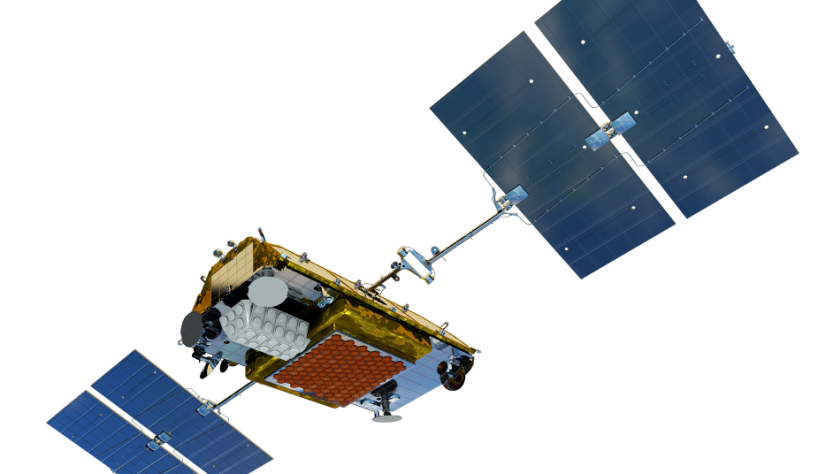
\includegraphics[width=13cm]{pic/IMG_Iridium-Satellite_NEXT-Satellite-Vehicle_HR_FEB16-clip-833x474.png}
\caption{第二代“铱星”卫星}
\label{fig:IMG_Iridium-Satellite_NEXT-Satellite-Vehicle}
\end{figure}

\begin{figure}[htbp]
\centering
\begin{minipage}[t]{0.48\textwidth}
\centering
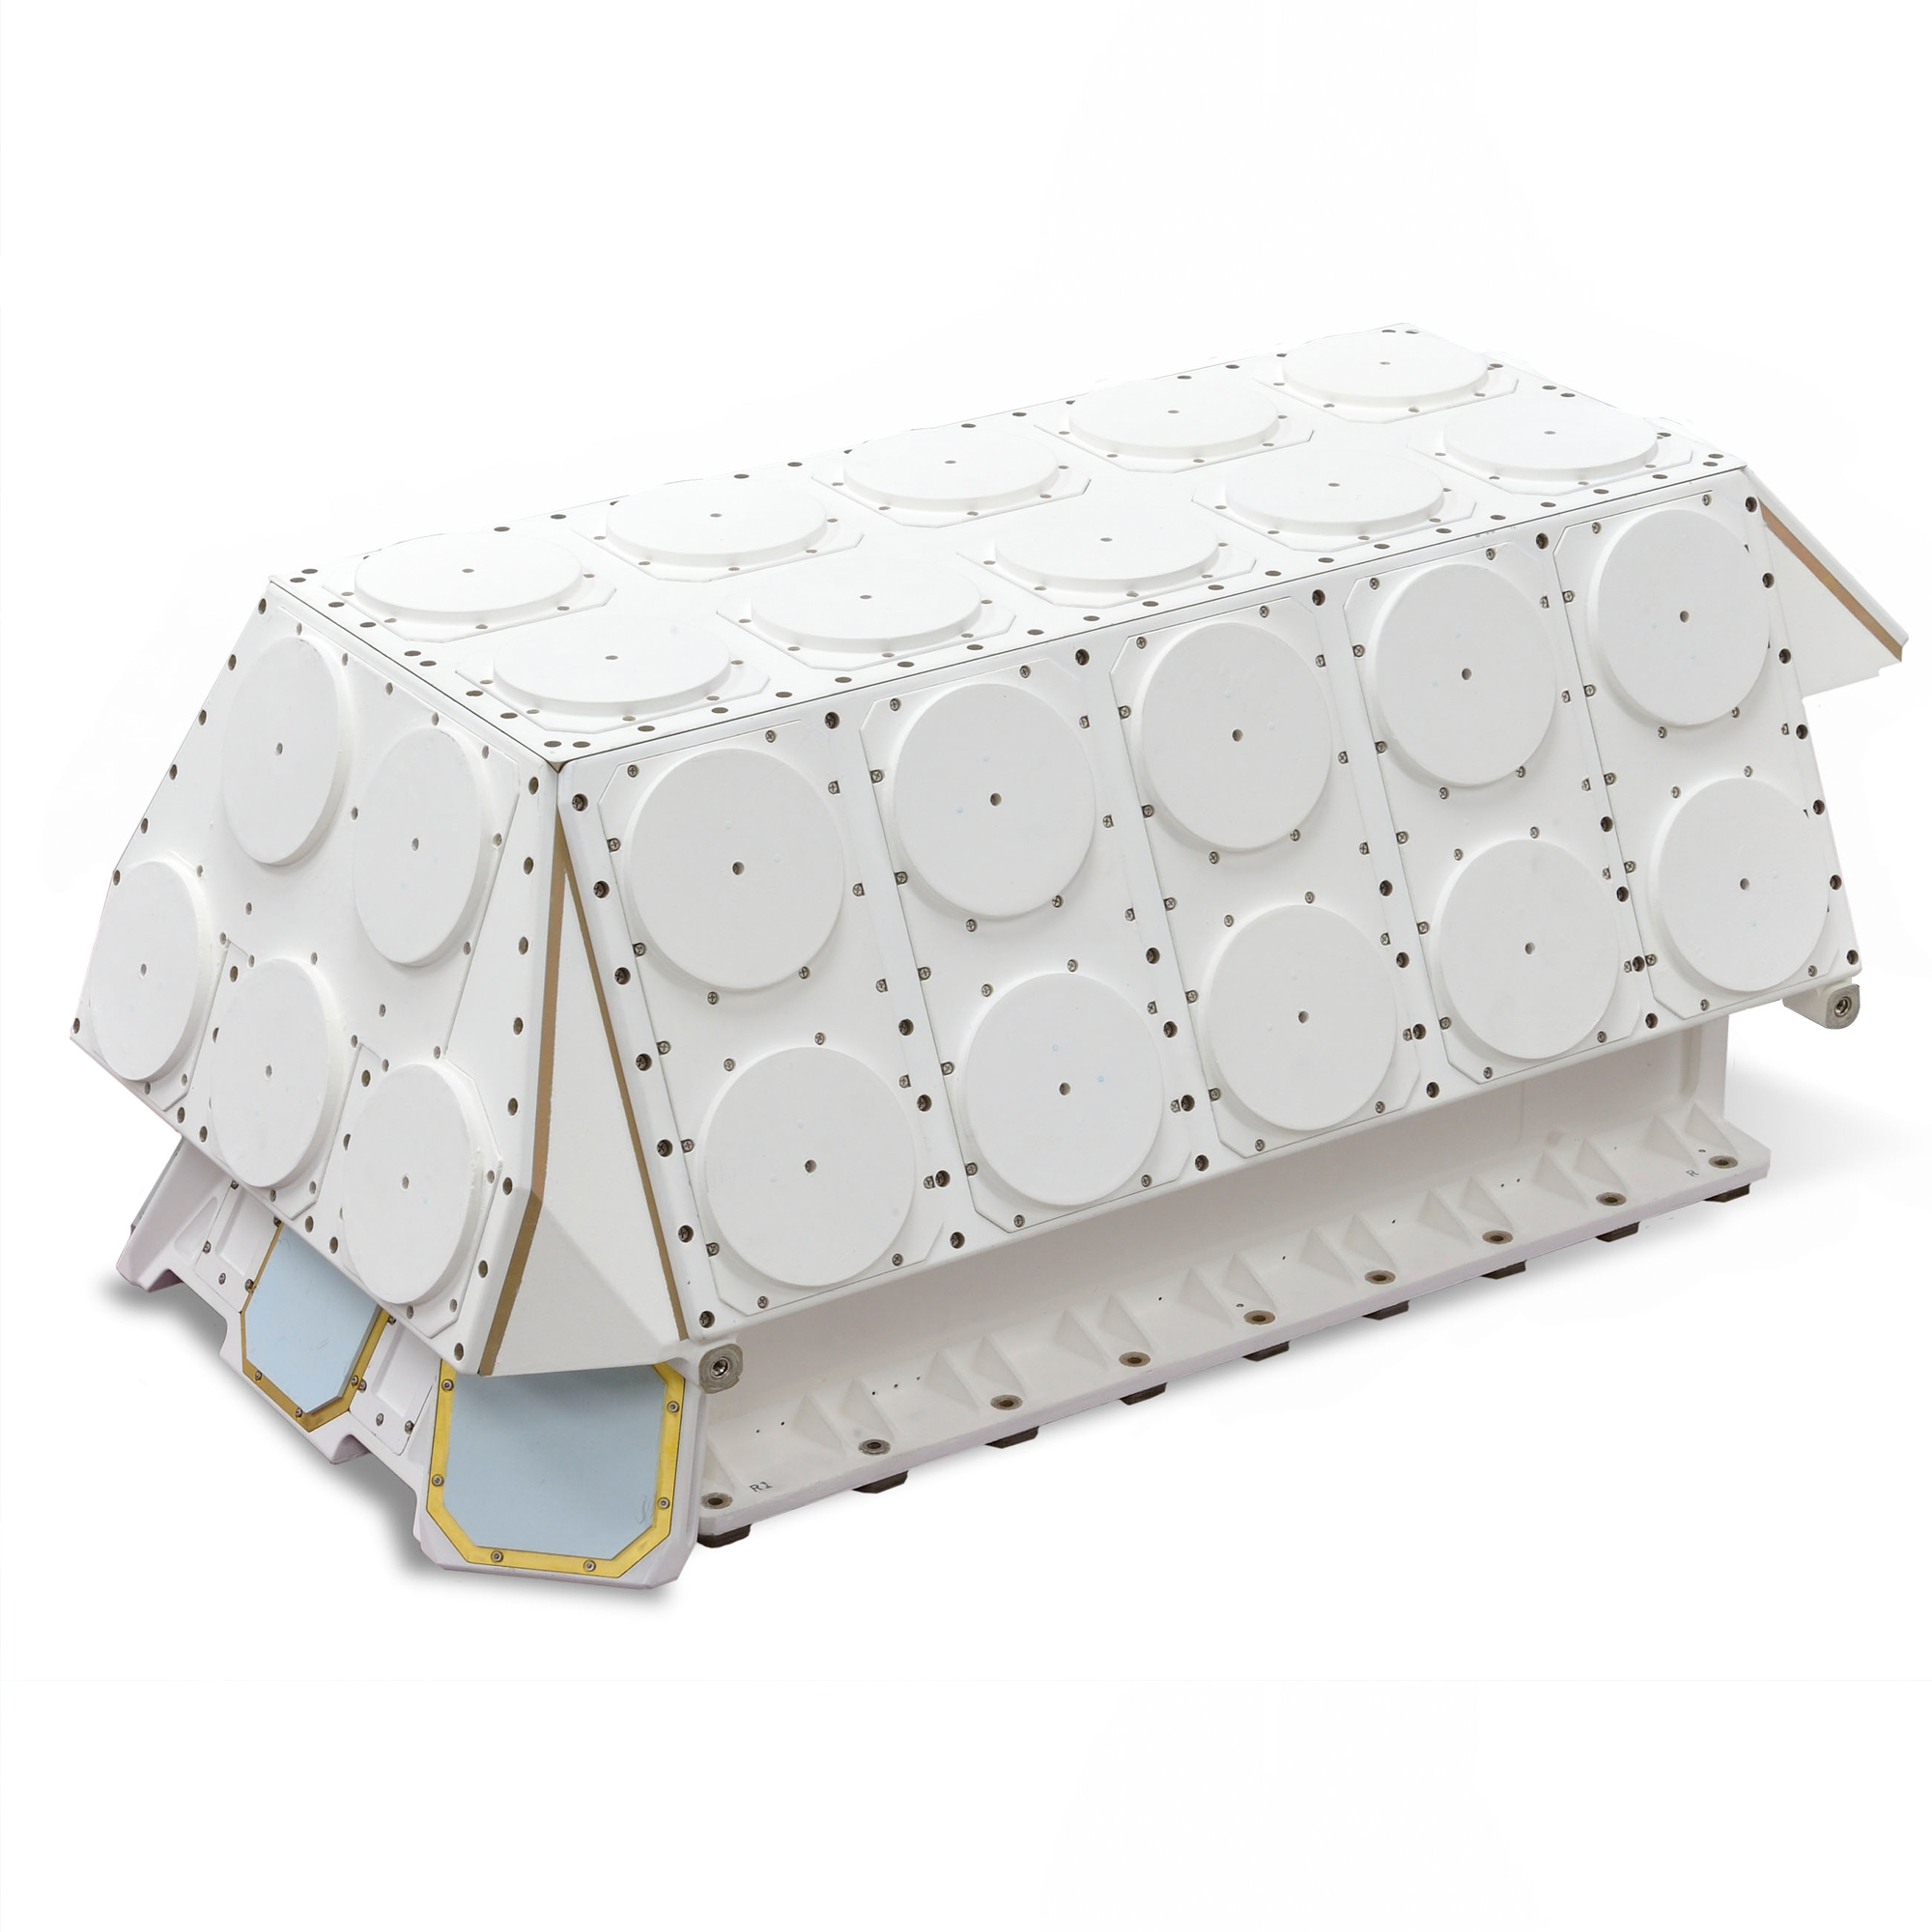
\includegraphics[width=6.5cm]{pic/Appstar_with_Base_2000x2000.jpg}
\caption{ADS-B 载荷}
\label{fig:Appstar_with_Base}
\end{minipage}
\begin{minipage}[t]{0.48\textwidth}
\centering
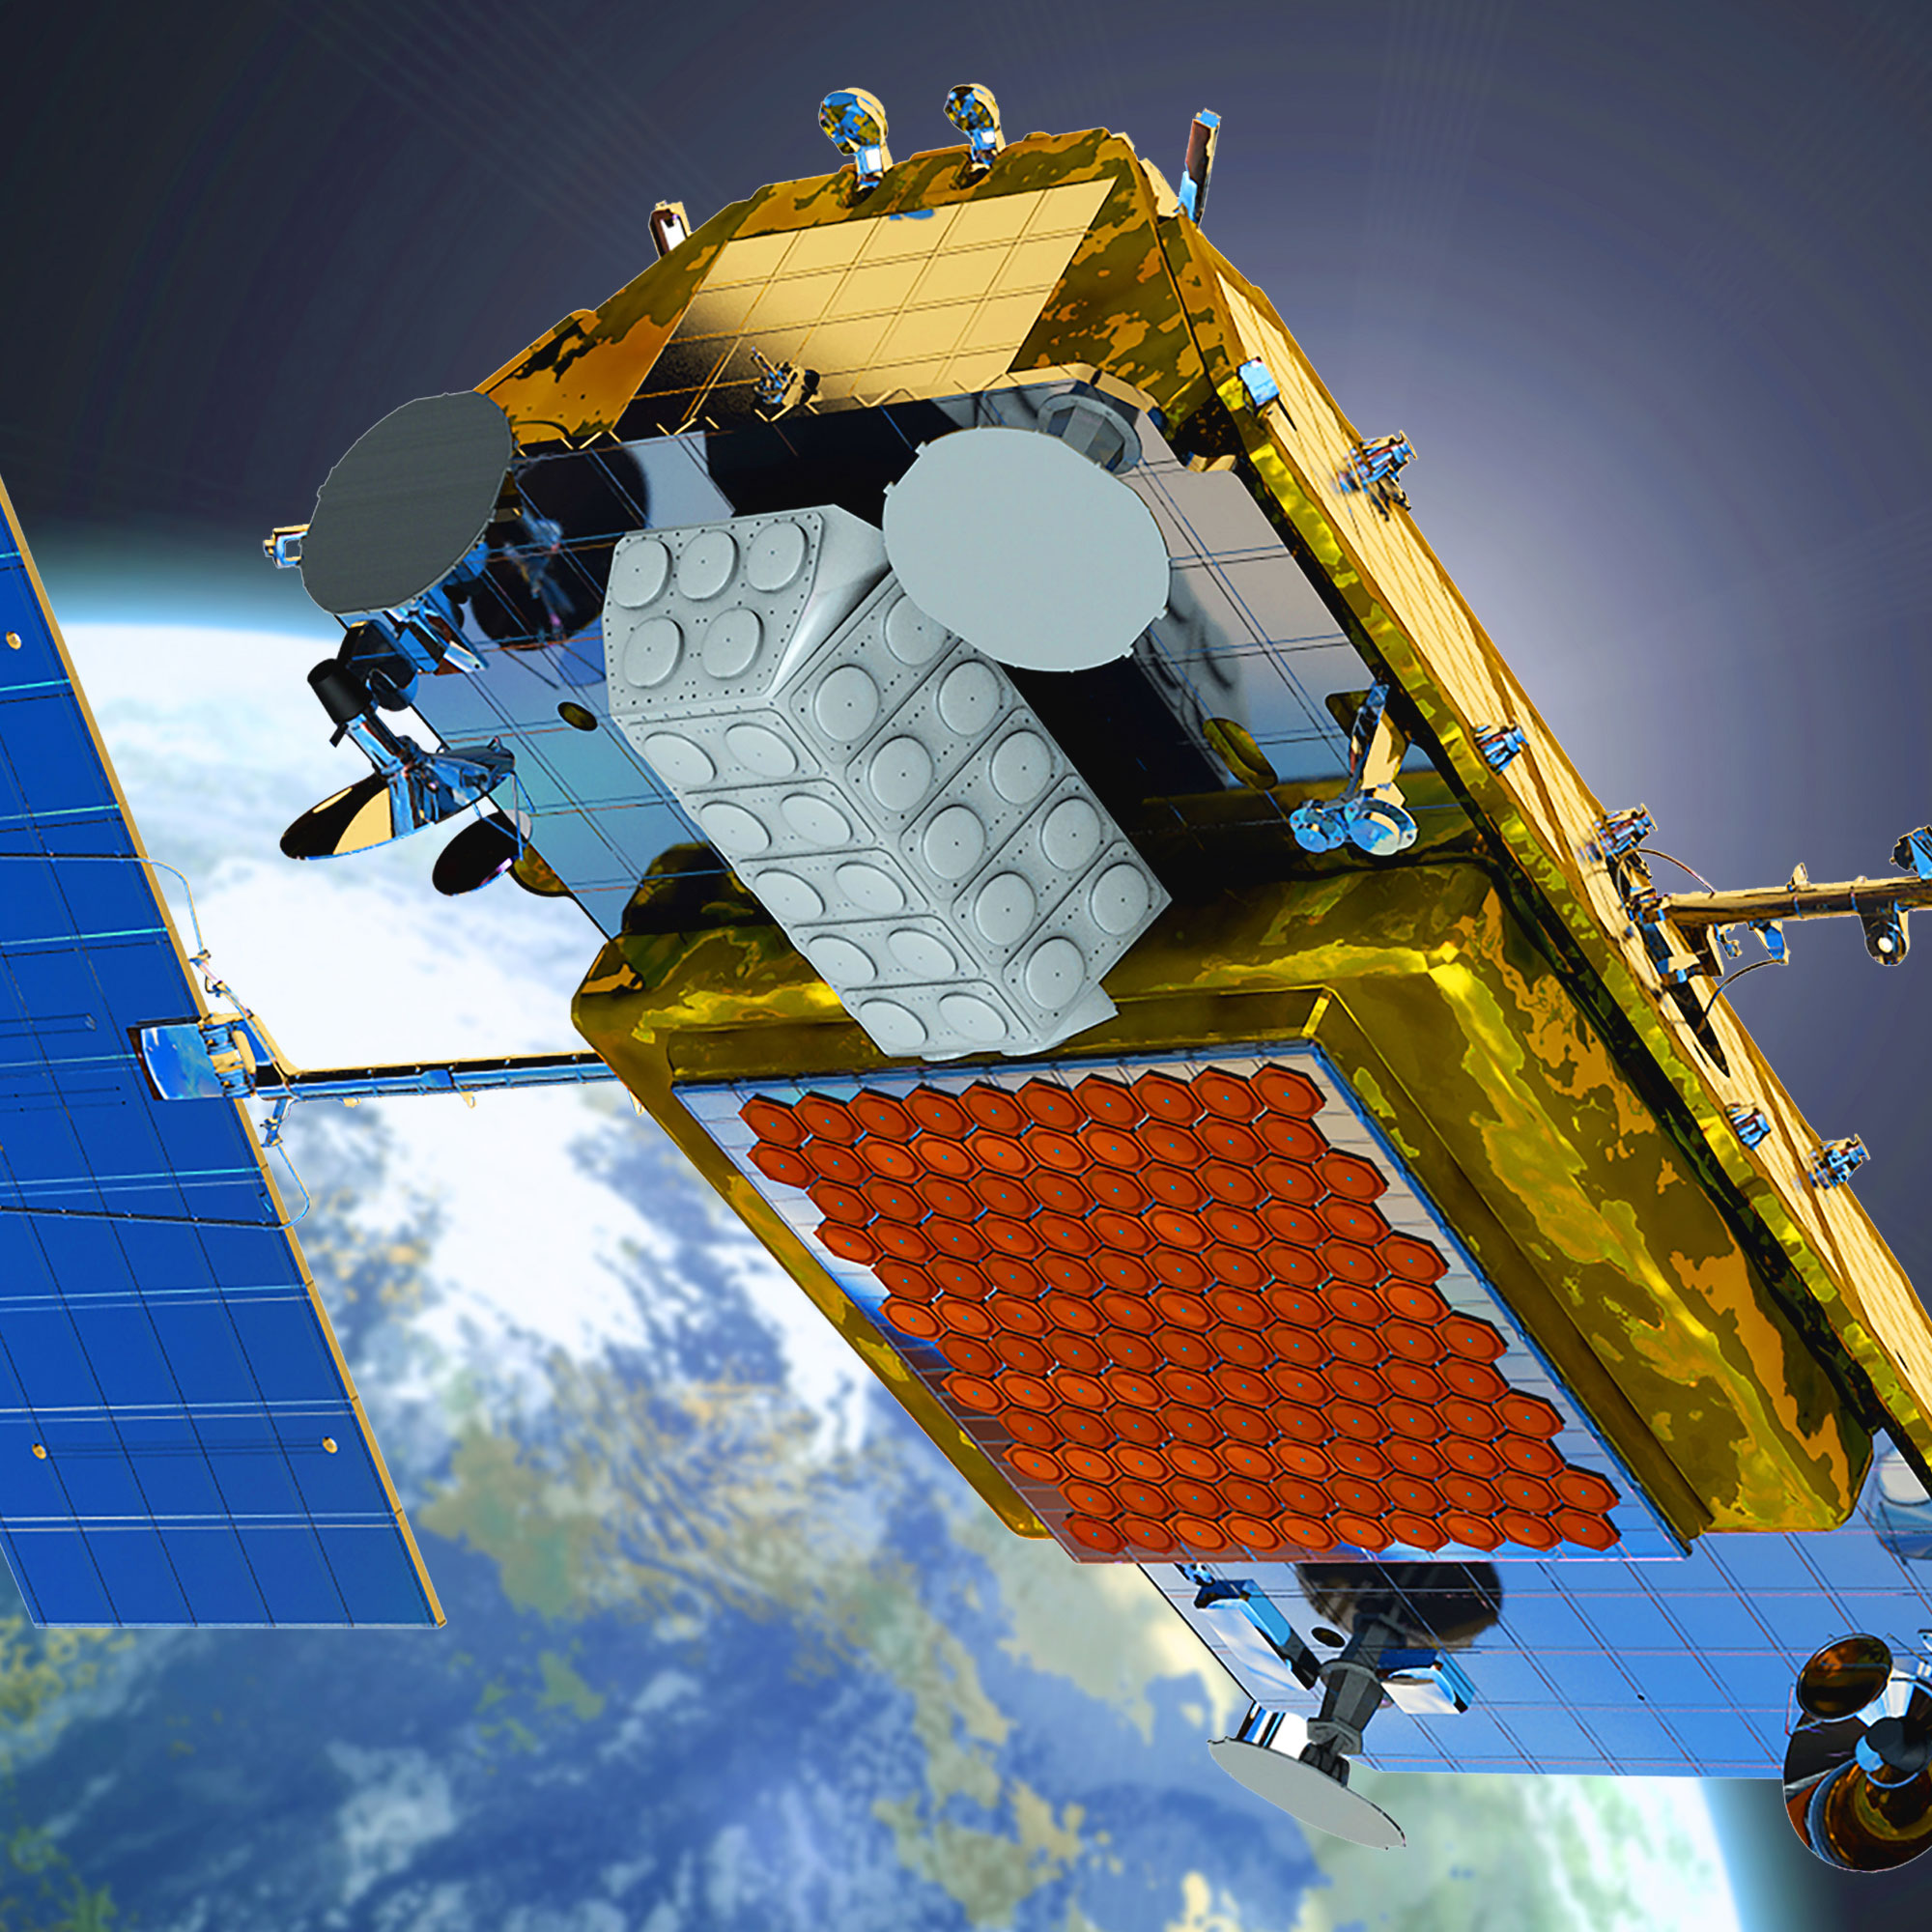
\includegraphics[width=6.5cm]{pic/reconfigurable_multimission_payloads_v2_web.jpg}
\caption{ADS-B 载荷搭载方式}
\label{fig:reconfigurable_multimission_payloads}
\end{minipage}
\end{figure}

\subsection{体系结构}

\subsection{系统性能}

\section{ALAS 系统}

\subsection{系统概述}

根据\url{www.ads-b.com}网站给出的说法,他们将天基 ADS-B 系统称为 ADS-B 链路增强系统(ADS-B Link Augmentation System),简称为“ALAS”。通过该系统,地球上任何地方的任意一架飞机可以被实时地安全追踪。

\subsection{体系结构}

\subsection{系统性能}

依托“全球星二代”系统的 ALAS 系统端到端(end-to-end)测试性能数据如表\ref{tab:alas-paras}所示。 \footnote{数据来源:\url{http://www.ads-b.com/space-based.htm}}

\renewcommand\arraystretch{1.5}
\begin{table}[htbp]
\centering
\caption{使用全球星卫星的 ALAS 系统端到端测试性能}
\label{tab:alas-paras}
\begin{tabular}[b]{|p{4cm}<{\raggedleft}|p{11cm}<{\raggedright}|}
\hline
\textbf{适用性
(Applicability)} &
ALAS 是一种简单、质量轻、低成本的外围设备,可与现有的任何 1090ES 或 UAT 电子设备配合使用,保证正常的空-地和地-空 ADS-B 传输不会中断。ALAS 还旨在与任何国家现有的 ADS-B 地面基础设施兼容\\
\hline
\textbf{覆盖范围(
Coverage Area)} &
到 2016 年,100\% 覆盖美国本土(CONUS)、GOMEX、加勒比海(Caribbean)、北大西洋(NAT)和北太平洋(NOPAC);到 2019 年,100\% 覆盖剩余地区\\
\hline
\textbf{可用性(
Availability)} & 到 2016 年,可用性为 99.99\%;到 2019 年,可用性为 99.999\% \\
\hline
\textbf{容量(
Capacity) }& 每架卫星可容纳大于 3000 架飞机(approx 1,800sm diameter)\\
\hline
\textbf{时延(
Latency)} &  从飞机到地面小于 200 毫秒;从端到端小于 300 毫秒 \\
\hline
\textbf{更新率(
Update Rate)} & 1 秒 \\
\hline
\textbf{完整性(
Integrity)} & 10E-6 \\
\hline
\textbf{精度(
Accuracy)} &
UTC 时制下,在 98\% 的时间里,相同目标的 射频视距(RF line-of-sight)导出位置和天基 ALAS 导出位置之间的显示位置差异小于 50 英尺\\
\hline
\textbf{安全性(
Security)} & 独一无二的安全。ALAS 与每架飞机建立了独特的双向连接,可以抵抗入侵、干扰或欺骗,是唯一的可以轻松加密的 ADS-B 形式。简单的防篡改设计还可以包括一个自供电备用系统,该系统将在未经授权而关闭飞机的主 ADS-B 转发器的情况下继续广播飞机的位置 \\
\hline
\textbf{可扩展性(
Scalability)}  & 高。系统架构的成本相对较低且简单,通过增加更多卫星和/或地面站,可以提高覆盖范围,可用性和容量 \\
\hline
\textbf{部署(
Deployment)} & 马上准备好。该技术已经过超过 100 小时的飞行测试。Globalstar 在过去两年中发射了 24 颗新的第二代 ALAS 卫星。Essential Services could be deployed as early as 3Q2016 and Critical Services NLT 2019\\
\hline
\textbf{成本(
Cost)} & 低。由于 ALAS 不需要新的卫星或太空中的其他技术,因此 ANSP 的买入和重复成本很小。它还可以与现有的 ADS-B 地面基础设施轻松连接。The price point for Part 121 avionics is less than \$40k and installation should be in the 20-25 MH range for most commercial aircraft. \\
\hline
\end{tabular}

\end{table}